\documentclass{article}
\usepackage[a4paper,left=2cm,right=2cm,top=2cm,bottom=2cm]{geometry}
\usepackage[utf8]{inputenc}  
\usepackage[T1]{fontenc}
\usepackage[french]{babel}
\usepackage{amsmath}
\usepackage{amsfonts}
\usepackage{dsfont}
\usepackage{graphicx}
\usepackage{caption}
\usepackage{listings}
\usepackage{svg}
\usepackage{pdfpages}
\usepackage{algorithmic}
\usepackage[hidelinks]{hyperref}
\setlength{\parindent}{0pt}
\setlength{\parskip}{1ex plus 0.5ex minus 0.2ex}
\newcommand{\hsp}{\hspace{20pt}}
\newcommand{\HRule}{\rule{\linewidth}{0.5mm}}
\newcommand*{\logeq}{\ratio\Leftrightarrow}

\title{Projet IA - Problème de la patrouille - Approche EVAP}
\author{Timothé Rios - Nicolas Venot}
\date{mars 2021}

\begin{document}
\maketitle
\newpage
\tableofcontents
\newpage
\setlength{\parindent}{0pt}

\section*{Introduction}
    \paragraph{}Une patrouille est une mission impliquant une équipe de plusieurs individus dont l'objectif consiste à visiter en permanence les zones concernées d'un environnement, afin de le superviser, le contrôler ou le protéger efficacement.
    Un groupe de drones à la recherche de feux de forêt afin de contribuer à la conservation des écosystèmes, une équipe de robots aspirateurs à la recherche de saletés, des facteurs effectuant leur tournée quotidienne ou une escouade militaire sécurisant une zone sont autant d'exemples de patrouilles.
    L'exécution d'une telle tâche implique que tous les membres impliqués coordonnent efficacement leurs actions.
    
    Dans ce rapport, nous étudions l'approche d'évaporation des phéromones.
    Cette approche, inspirée par l'étude des colonies d'insectes sociaux, a pour 
    particularité d'attribuer à chaque zone géographique un taux de phéromones spécifique qui diminue avec le temps.
    Les agents ont alors pour fonction de maximiser autant que possible le taux de phéromones 
    des zones autour d'eux, d'où la nécessité de patrouiller et la pertinence de ce modèle pour 
résoudre ce problème.

\section{Principe général}

    \paragraph{} Dans ce modèle, le temps est discrétisé et l'environnement est modélisé par une grille de cases. Chaque agent
    avance d'une case par pas de temps, sur la case à gauche, à droite, devant ou derrière lui qui a la plus petite quantité de 
    phéromones. Chaque fois qu'un agent arrive sur une case, il dépose une quantité $P_{max}$ de phéromones sur celle-ci. 

    À chaque pas de temps, toutes les cases perdent une certaine quantité de phéromones : si elles ont $P_t$ phéromones
    à l'instant $t$, elles ont $P_{t+1} = P_t * (1-p)$ à l'instant $t+1$, avec $p$ compris entre $0$ et $1$ exclus.

    Une catégorie de cases ne peut pas recevoir de phéromones et ne peut pas être traversée par les agents. Cette catégorie permet
    de représenter des murs ou des obstacles dans ce modèle. Évidemment, les agents en contact avec des cases de type mur
    ne vont pas prendre en compte ces dernières dans leurs déplacements.

    Enfin, si plusieurs cases atteignables par un agent au prochain pas de temps ont toutes deux le niveau de phéromones minimum 
    parmi les voisins de cet agent, il choisit au hasard parmi celles-ci. Cependant, si une de ces cases est la case qui lui fait 
    face, il a la probabilité $p_{avant}$ de garder sa trajectoire. Ceci permet d'éviter des mouvements trop erratiques.

    Afin de pouvoir étudier l'efficacité du modèle en fonction des valeurs de ses différents paramètres, nous utilisons trois paramètres
    d'observation. Le premier est l'inoccupation instantanée de la case (INI pour \textit{Instantaneous  Node  Idleness }), un paramètre 
    spécifique à chaque case qui correspond au nombre de pas depuis la dernière visite de cette case par un agent. Le deuxième est 
    l'inoccupation instantanée du graphe (IGI pour \textit{Instantaneous  Graph  Idleness }), qui correspond à la moyenne des INI de toutes les
    cases à chaque pas. Enfin, le dernier paramètre d'observation que nous utilisons est l'inoccupation instantanée maximum (IWI pour 
    \textit{Instantaneous   Worst   Idleness }), qui correspond à l'INI maximum à chaque pas.

\section{Implémentation}
    \subsection{Les cases}

        \paragraph{}Chaque case se voit attribuer plusieurs paramètres.
Le premier est un booléen \texttt{mur} indiquant si la case est un mur ou non et le deuxième est un nombre \texttt{phéromone} indiquant le niveau de phéromones
        de la case. Le dernier paramètre est un entier \texttt{ini} qui recense l'INI de la case.

        Durant une simulation, le \texttt{phéromone} de chaque case diminue à chaque pas de temps comme expliqué plus-haut : $p$, le coefficient
        d'évaporation, est un paramètre réglable de la simulation mais n'a qu'une influence esthétique. les cases ayant leur paramètre \texttt{mur}
        à \texttt{true} ne font pas diminuer la valeur de leur \texttt{phéromone} et ne font pas augmenter leur \texttt{ini}, qui ne sont de toute façon jamais pris en compte dans la simulation.
        la couleur des cases varie en fonction de leur état de mur ou non et de leur niveau de phéromones : les cases
        ayant le booléen \texttt{mur} à \texttt{true} sont bleues et les autres ont une couleur verte dont l'intensité varie proportionnellement à leur
        niveau de phéromones.
    \subsection{Les agents}
        \paragraph{}À chaque pas de temps, les agents se déplacent sur la case mitoyenne (uniquement sur la même ligne ou sur la même colonne) 
        ayant le paramètre \texttt{phéromone} le plus bas et l'incrémente de \textit{un}. Ce faisant, il remet aussi le paramètre \texttt{ini} 
        de la case à \textit{zéro}. Les agents ignorent les cases ayant leur paramètre \texttt{mur} à \texttt{true}. Tous les agents ont la 
        même probabilité \texttt{p\_avant} de privilégier la case devant eux si celle-ci fait partie des cases mitoyennes ayant la valeur minimum
        de \texttt{phéromone}.
\section{Algorithme}
    \subsection{Algorithme des cases}
    \begin{algorithmic}
        \FOR {chaque case $c$}
        \IF {$c$ n'est pas un mur} 
            \STATE $c.ph$\textit{é}$romone \gets c.ph$\textit{é}$romone  * (1-p)$
            \STATE $c.ini \gets c.ini+1$
        \ENDIF 
        \ENDFOR
        \end{algorithmic}
    \subsection{Algorithme des agents}
    \begin{algorithmic}
        \FOR{chaque agent $a$}
            \STATE $voisins\_min \gets \{\,\}$
            \STATE $min \gets $minimum du phéromone des voisins
            \FOR{chaque case voisine $v$ de $a$}
                \IF {$v$ n'est pas un mur et $v.ph$\textit{é}$romone$ = $min$}
                    \STATE $voisins\_min \gets voisins\_min + v$
                \ENDIF
            \ENDFOR
            \STATE $case\_devant \gets$ case en face de l'agent
            \IF {$case\_devant$ est dans $voisins\_min$ et $random(1) < p$}
                \STATE  $case\_prochaine \gets case\_devant$
            \ELSE
                \STATE $case\_prochaine \gets random(voisins\_min)$
            \ENDIF
            \STATE l'agent va sur $case\_prochaine$
        \ENDFOR
    \end{algorithmic}
\section{Étude des paramètres}
    \subsection{Présentation des différents environnements}
        \paragraph{} Afin de comparer l'effet des différents paramètres de notre modèle, nous avons effectué plusieurs simulations sur différents environnements.
        Le premier est une grille carrée de vingt cases par vingt cases, dont toutes les cases sont accessibles aux agents.

        Le deuxième est une grille de même dimension mais contenant une spirale de cases obstacles.

        Le dernier est une grille rectangulaire de vingt cases par vingt-cinq contenant un couloir centrale menant à six pièces, formées par des cases obstacles.
        
        \begin{figure}[!h]
            \begin{center}
                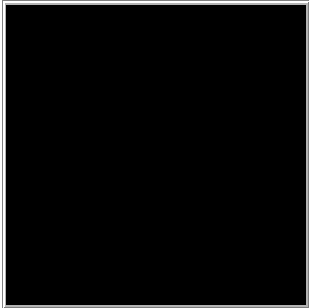
\includegraphics[width = \textwidth/5]{defaut_png.PNG}
                
\includegraphics[width = \textwidth/5,]{spirale_png.PNG}
                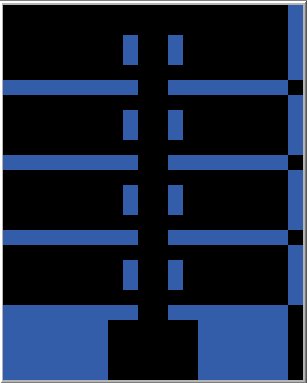
\includegraphics[width = \textwidth/5, height = 3.7cm]{corridor_png.PNG}
                \caption{Environnements de test \\ \textit{les obstacles sont en bleu, les cases normales en noir}}
            \end{center}
        \end{figure}

        \paragraph{} Nous allons donc étudier les effets de deux paramètres : le nombre d'agents et la probabilité d'aller tout droit.
    \subsection{Nombre d'agents}
        \paragraph{}Évidemment, l'efficacité de la patrouille augmente à mesure que l'on ajoute des agents.
        \subsubsection{Environnement vide}
            \paragraph{} On remarque sur les deux graphes de l'IGI et l'IWI que la valeur moyenne de ces deux paramètres est inversement proportionnelle au nombre d'agents.
            Notamment, si l'on double le nombre d'agents, on diminue de moitié les moyennes de l'IGI et de l'IWI. Néanmoins, les valeurs maximales de ces deux paramètres ne suivent pas la même règle.
            Même si la tendance reste la même, on peut remarquer que l'aléatoire présent dans le modèle (au niveau du choix des agents de la case suivante) a des conséquences non négligeables sur les
            extrêmes.
            \begin{figure}[!h]
                \begin{center}
                    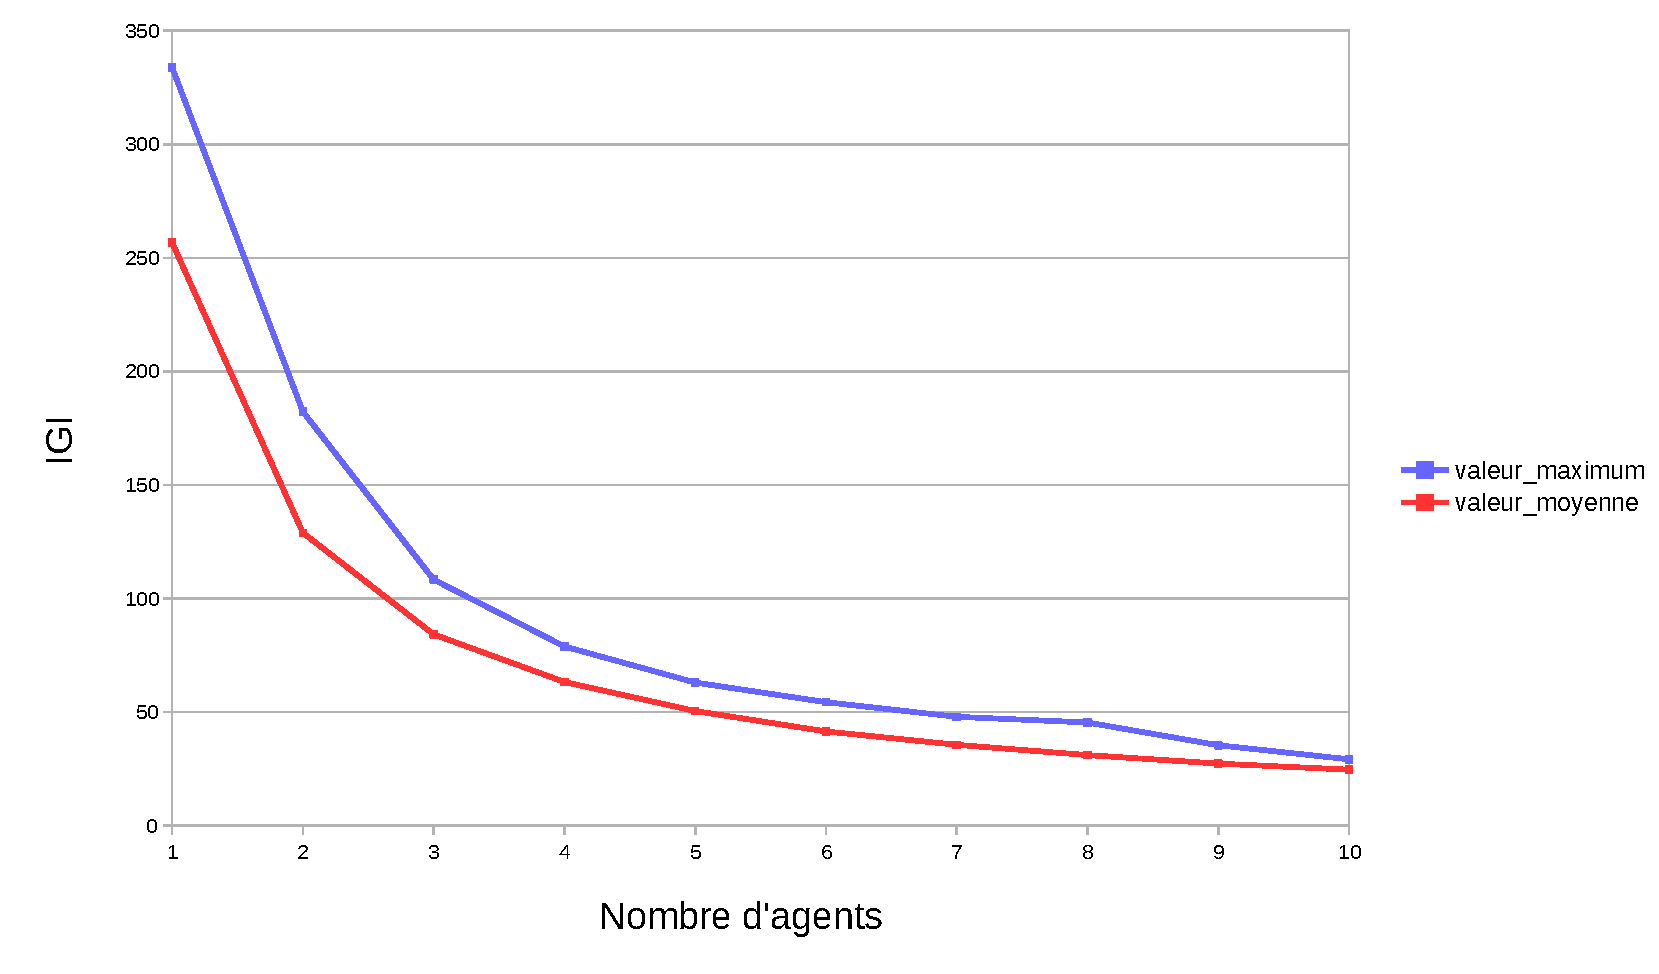
\includegraphics[height = 8.1 cm]{graphes pdf/variance tortues IGI.pdf}
                    \caption{IGI en fonction du nombre d'agents pour l'environnement vide}
                \end{center}
            \end{figure}
            \begin{figure}[!h]
                \begin{center}
                    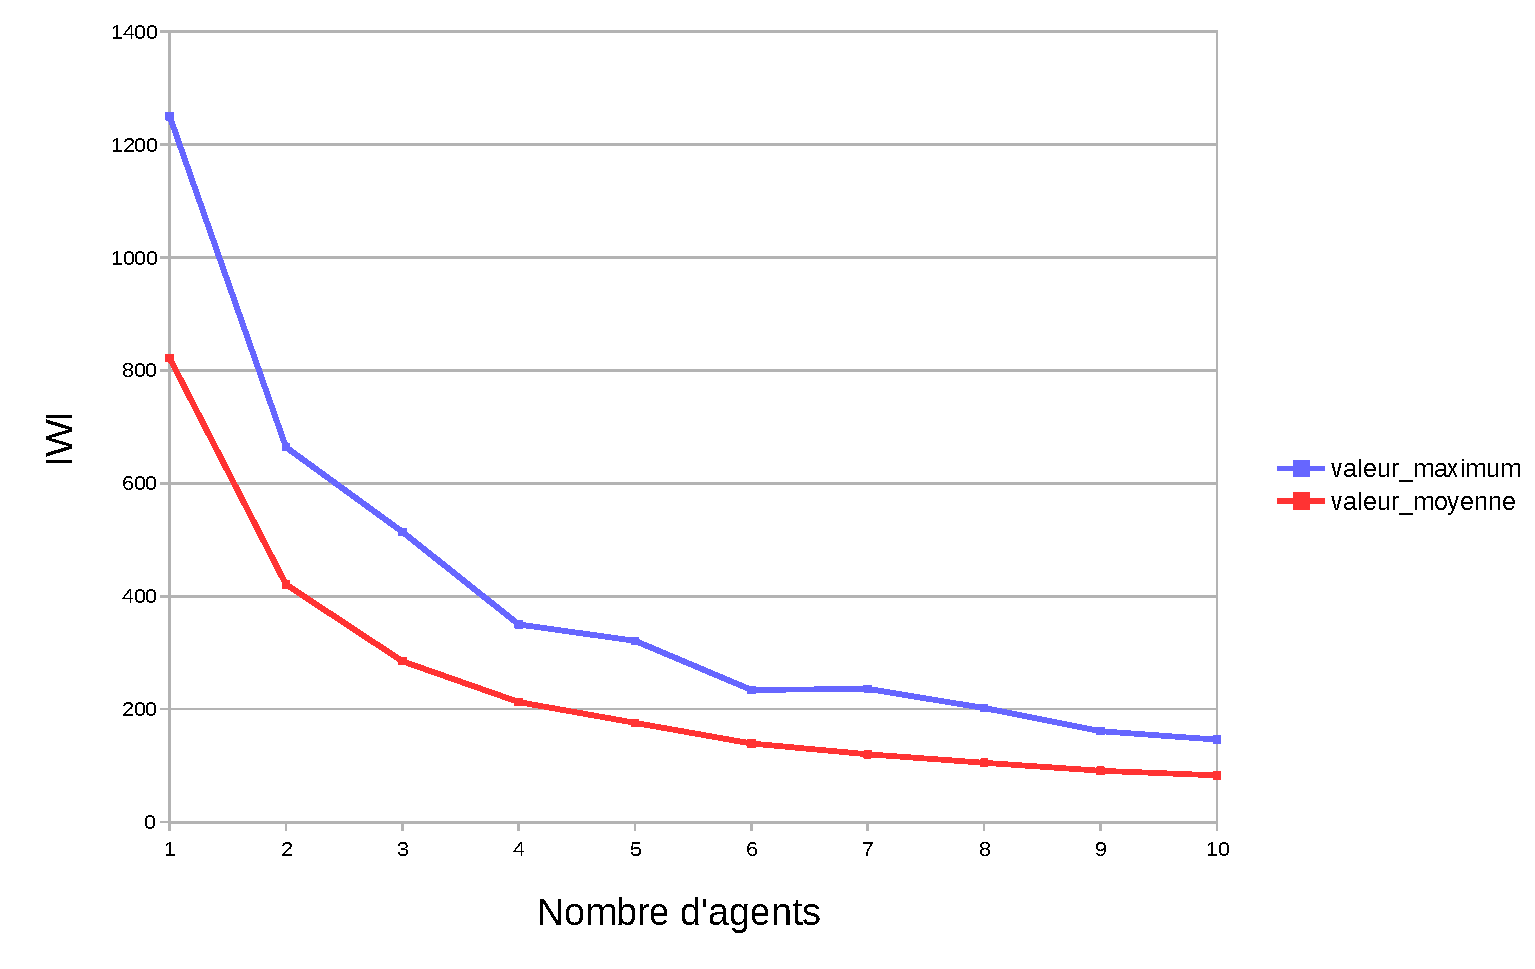
\includegraphics[height = 8.1cm]{graphes pdf/variance tortues IWI.pdf}
                    \caption{IWI en fonction du nombre d'agents pour l'environnement vide}
                \end{center}
            \end{figure}
            \newpage
        \subsubsection{Environnement en spirale}
        \paragraph{} Contrairement à l'environnement vide, le nombre d'agents dans l'environnement en spirale n'est pas parfaitement inversement proportionnelle aux taux d'IGI et d'IWI.
        Par exemple, on peut noter sur le graphique que passer de un à deux agents fait baisser l'IGI moyenne d'environ 62 \%, Contrairement aux 50 \% auquel on pourrait s'attendre.
        On remarque également que l'écart entre les maximums et les moyennes des valeurs est beaucoup plus élevé que dans l'environnement vide. Ainsi, le maximum d'IWI dans l'environnement vide à un agent valait 1,5 fois la valeurs de la moyenne, tandis qu'avec un agent dans l'environnement en spirale, le maximum d'IWI est 4,4 fois supérieur à sa moyenne.
        Enfin, on peut noter que les valeurs maximum de l'IGI et de l'IWI pour trois et quatre agents sont plus élevées que celles pour deux agents, ce qui montre que l'aléatoire a un plus grand impact sur cet environnement que sur le précédent.
            \begin{figure}[!h]
                \begin{center}
                    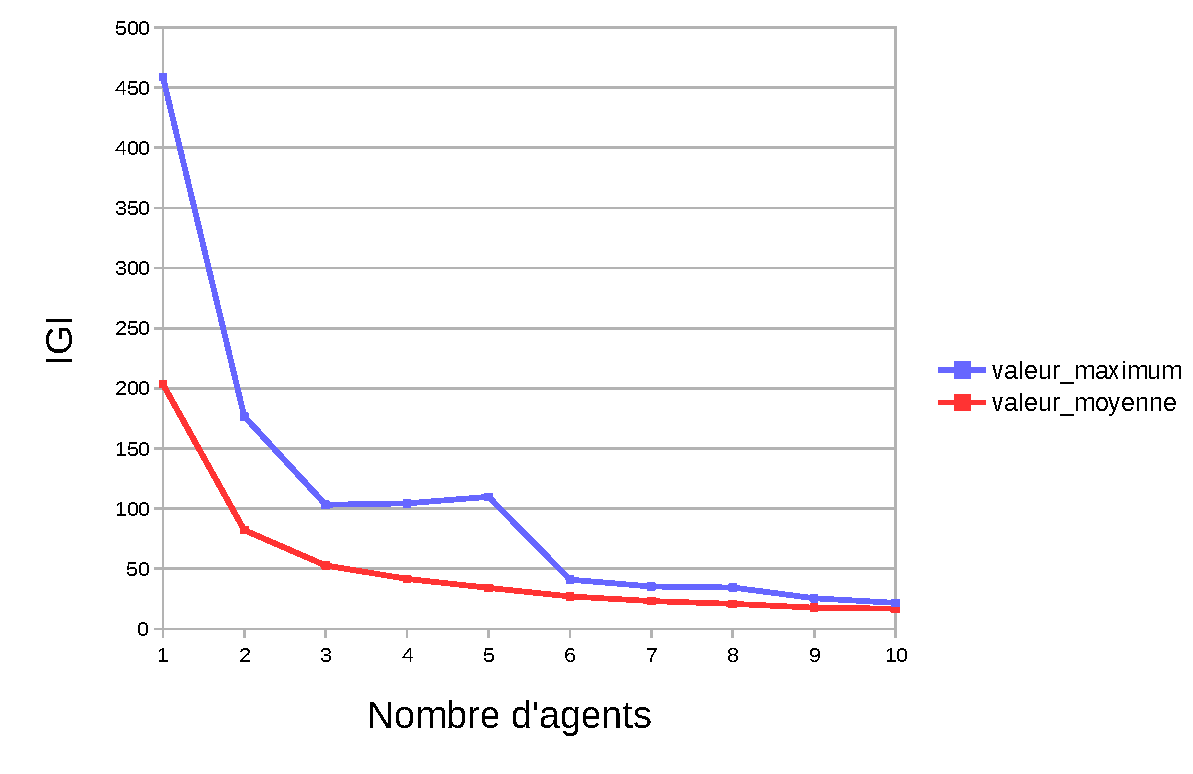
\includegraphics[width = 0.82\textwidth]{graphes pdf/variance tortues IGI spirale.pdf}
                    \caption{IGI en fonction du nombre d'agents pour l'environnement en spirale}
                \end{center}
            \end{figure}
            \begin{figure}[!h]
                \begin{center}
                    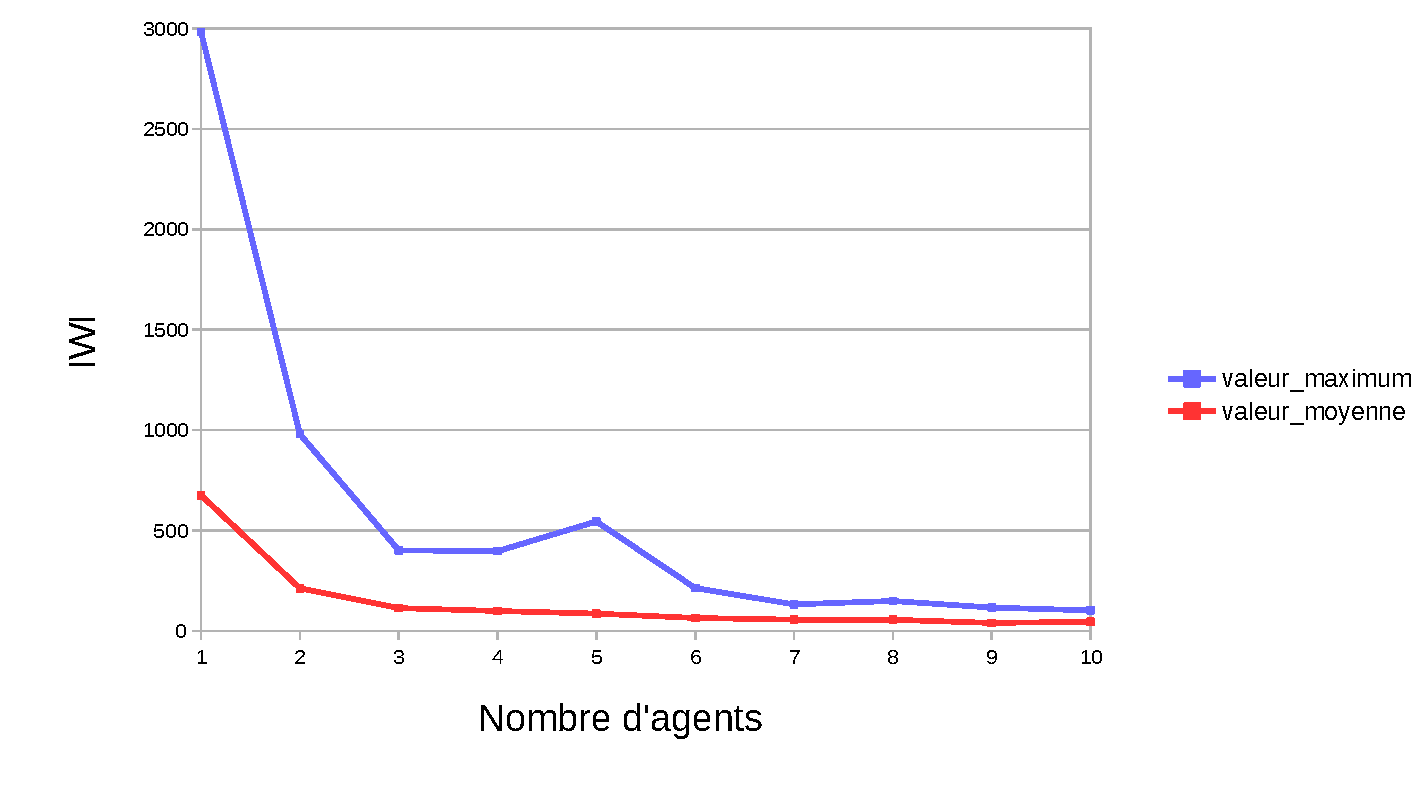
\includegraphics[width = 0.82\textwidth]{graphes pdf/variance tortues IWI spirale.pdf}
                    \caption{IWI en fonction du nombre d'agents pour l'environnement spirale}
                \end{center}
            \end{figure}
            \newpage
        \subsubsection{Environnement en corridor}
            \paragraph{} Contrairement à l'environnement en spirale, où passer de un à deux agents était plus avantageux que ce à quoi on aurait pu s'attendre, passer de un à deux agents sur l'environnement en corridor ne donne qu'une baisse de 40 \% pour l'IGI moyenne et de 20 \% pour l'IWI moyenne.
            De même, passer de deux à quatre agent ne fait baisser l'IWI que de 44 \% mais divise bien l'IGI moyen par deux. La disposition en corridor a donc pour effet de diminuer l'avantage apporté par des agents supplémentaires lorsque le nombre d'agents est faible.
            On remarque aussi que les valeurs maximum des deux paramètres peuvent croître en même temps que le nombre d'agents. Cette configuration en corridor a ainsi un risque important de comporter des cases qui ne sont pas visitées pendant un grand nombre de pas proportionnellement au nombre d'agents, quelque soit ce dernier.

            \begin{figure}[!h]
                \begin{center}
                    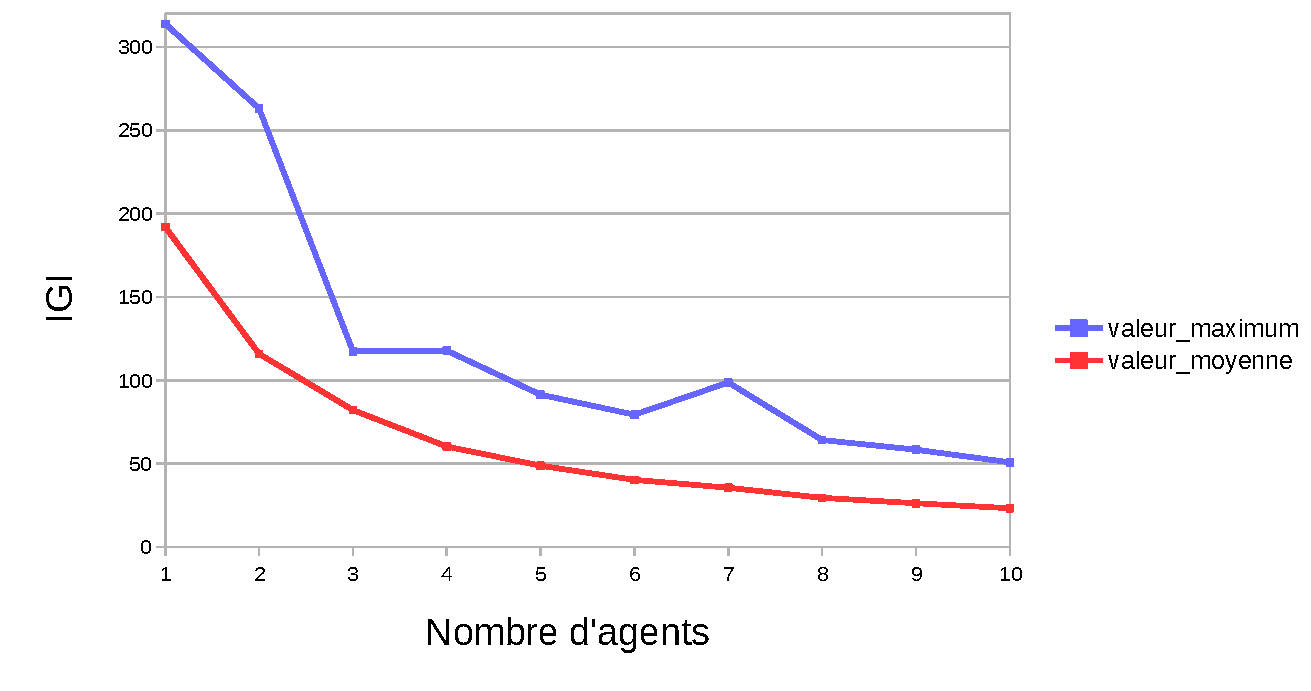
\includegraphics[width = 0.82\textwidth]{graphes pdf/variance tortues IGI corridor.pdf}
                    \caption{IGI en fonction du nombre d'agents pour l'environnement en corridor}
                \end{center}
            \end{figure}
            \begin{figure}[!h]
                \begin{center}
                    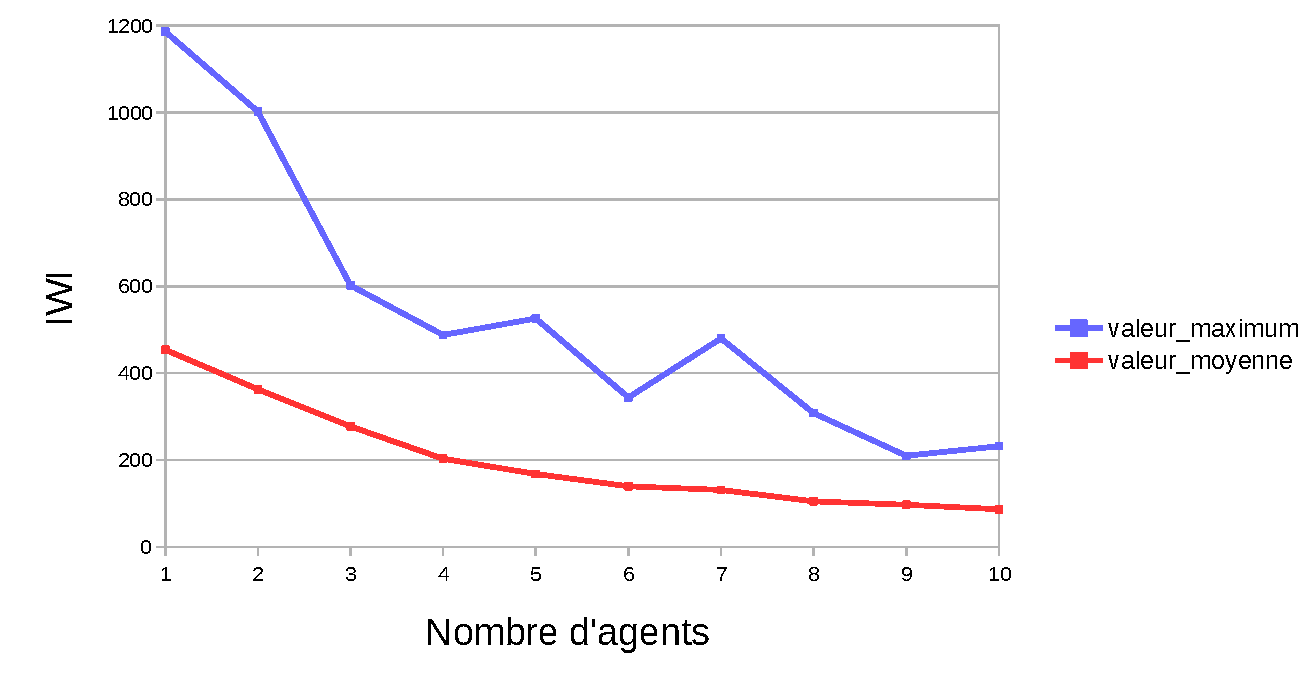
\includegraphics[width = 0.82\textwidth]{graphes pdf/variance tortues IWI corridor.pdf}
                    \caption{IWI en fonction du nombre d'agents pour l'environnement en corridor}
                \end{center}
            \end{figure}
            \newpage
    \subsection{Valeur de \texorpdfstring{$p_{avant}$}{p\_avant}}
    \paragraph{}Pour rappel, $p_{avant}$ détermine la probabilité qu'un agent donne la priorité à une case directement en face de lui si elle a le niveau le plus faible de chemical dans la proximité directe de l'agent.
    Dans le cas contraire, la case choisie va avoir un niveau de chemical minimal mais pas nécessairement celle faisant face à l'agent. 
    \subsubsection{Environnement vide}
    \paragraph{}On observe que les tendances moyennes d'IGI et d'IWI reste stable avec la variation de $p_{avant}$. Cet environnement étant dénué de mur, toutes les cases doivent être visitées pour limiter les valeurs maximales d'IWI et d'IGI.
    On n'observe donc aucune tendance particulière avec la variation de $p_{avant}$.
    \begin{figure}[!h]
        \begin{center}
            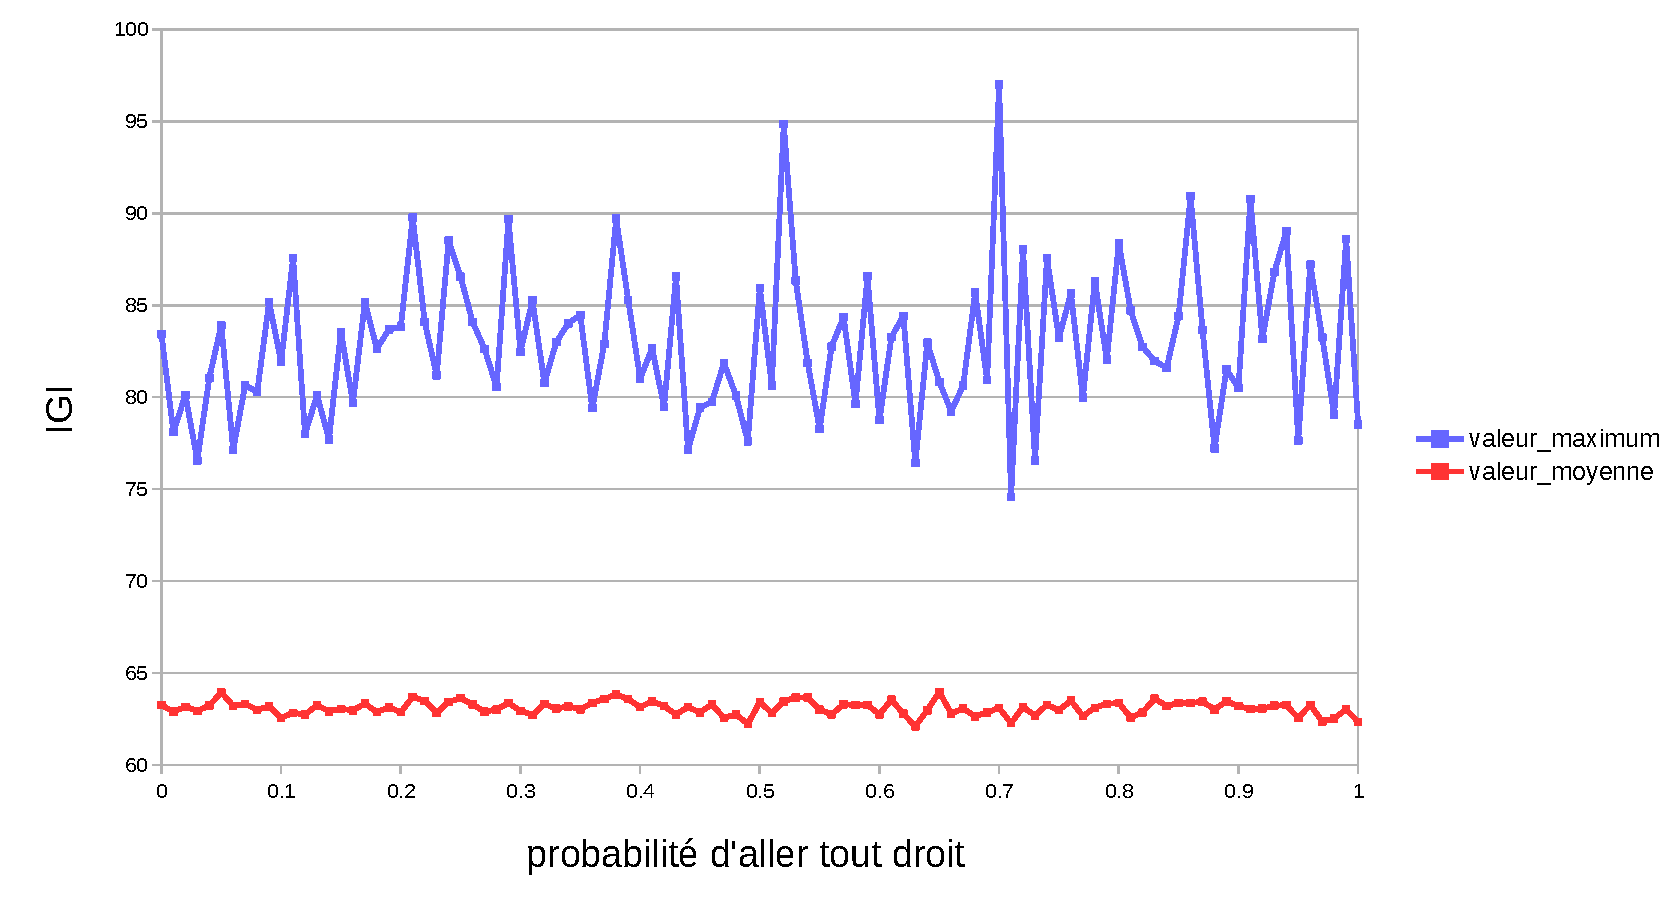
\includegraphics[width = 0.82\textwidth]{graphes pdf/variance go-ahead IGI.pdf}
            \caption{IGI en fonction de $p_{avant}$ pour l'environnement vide}
        \end{center}
    \end{figure}
    \begin{figure}[!h]
        \begin{center}
            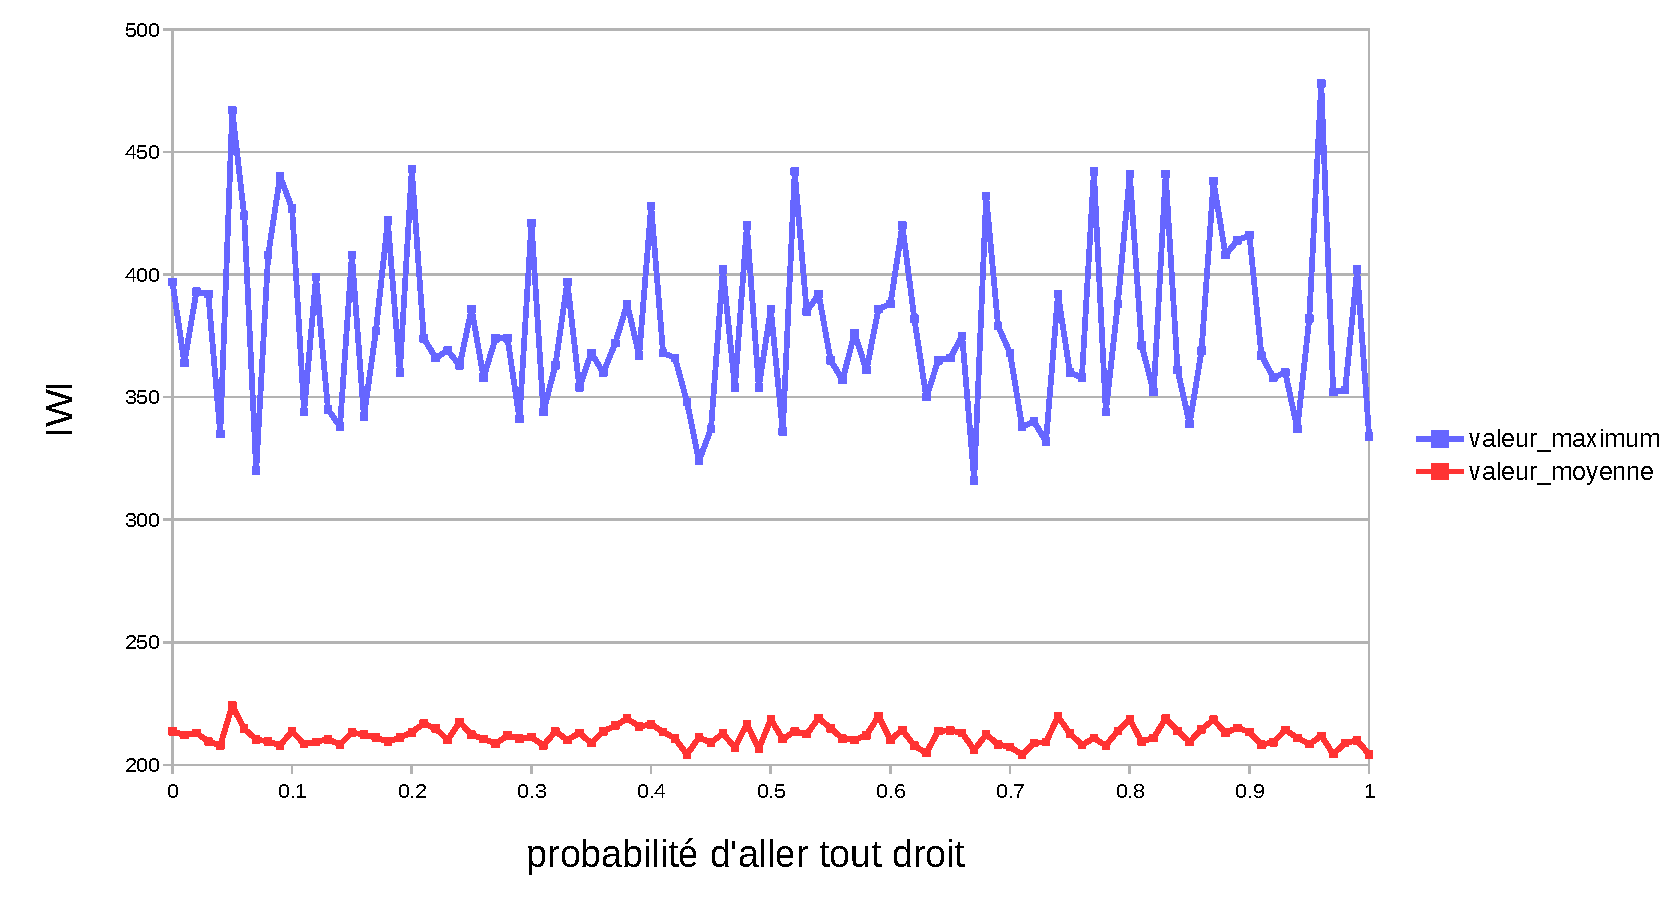
\includegraphics[width = 0.82\textwidth]{graphes pdf/variance go-ahead IWI.pdf}
            \caption{IWI en fonction de $p_{avant}$ pour l'environnement vide}
        \end{center}
    \end{figure}
    \newpage
    \subsubsection{Environnement en spirale}
    \paragraph{}On observe que les tendances moyennes d'IGI et d'IWI reste stable avec la variation de $p_{avant}$. Cependant, les valeurs maximales tendent à diminuer à mesure que la probabilité d'aller tout droit se rapproche de 1.
    Ceci peut s'expliquer par la forme spirale, qui demande d'être parcourue entièrement et donc d'atteindre le centre en effectuant le moins de détours possible pour avoir des valeurs d'IGI et d'IWI les plus basses.
    \begin{figure}[!h]
        \begin{center}
            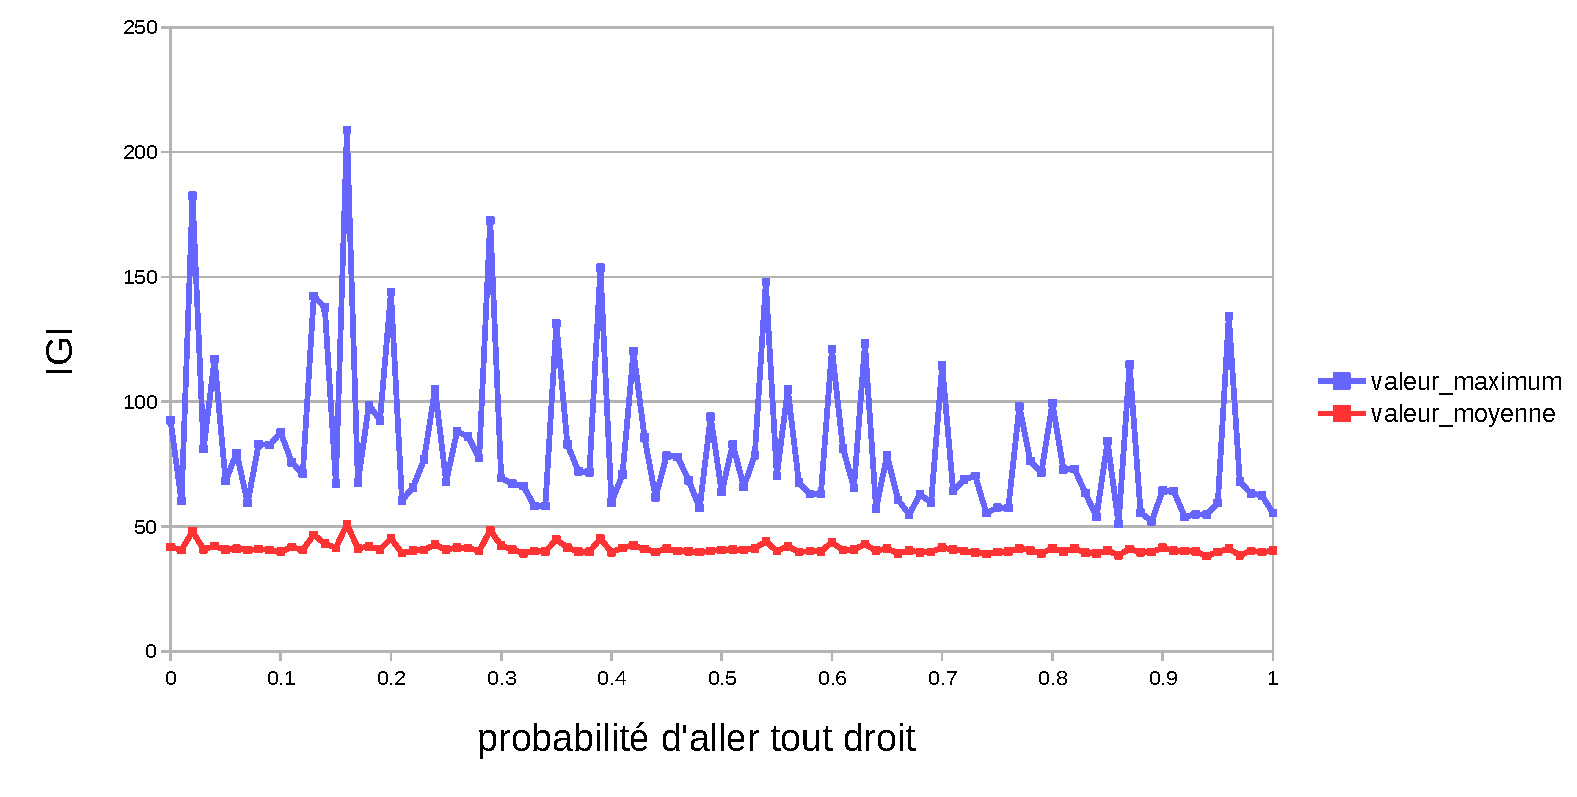
\includegraphics[width = 0.82\textwidth]{graphes pdf/variance go-ahead IGI spirale.pdf}
            \caption{IGI en fonction de $p_{avant}$ pour l'environnement en spirale}
        \end{center}
    \end{figure}
    \begin{figure}[!h]
        \begin{center}
            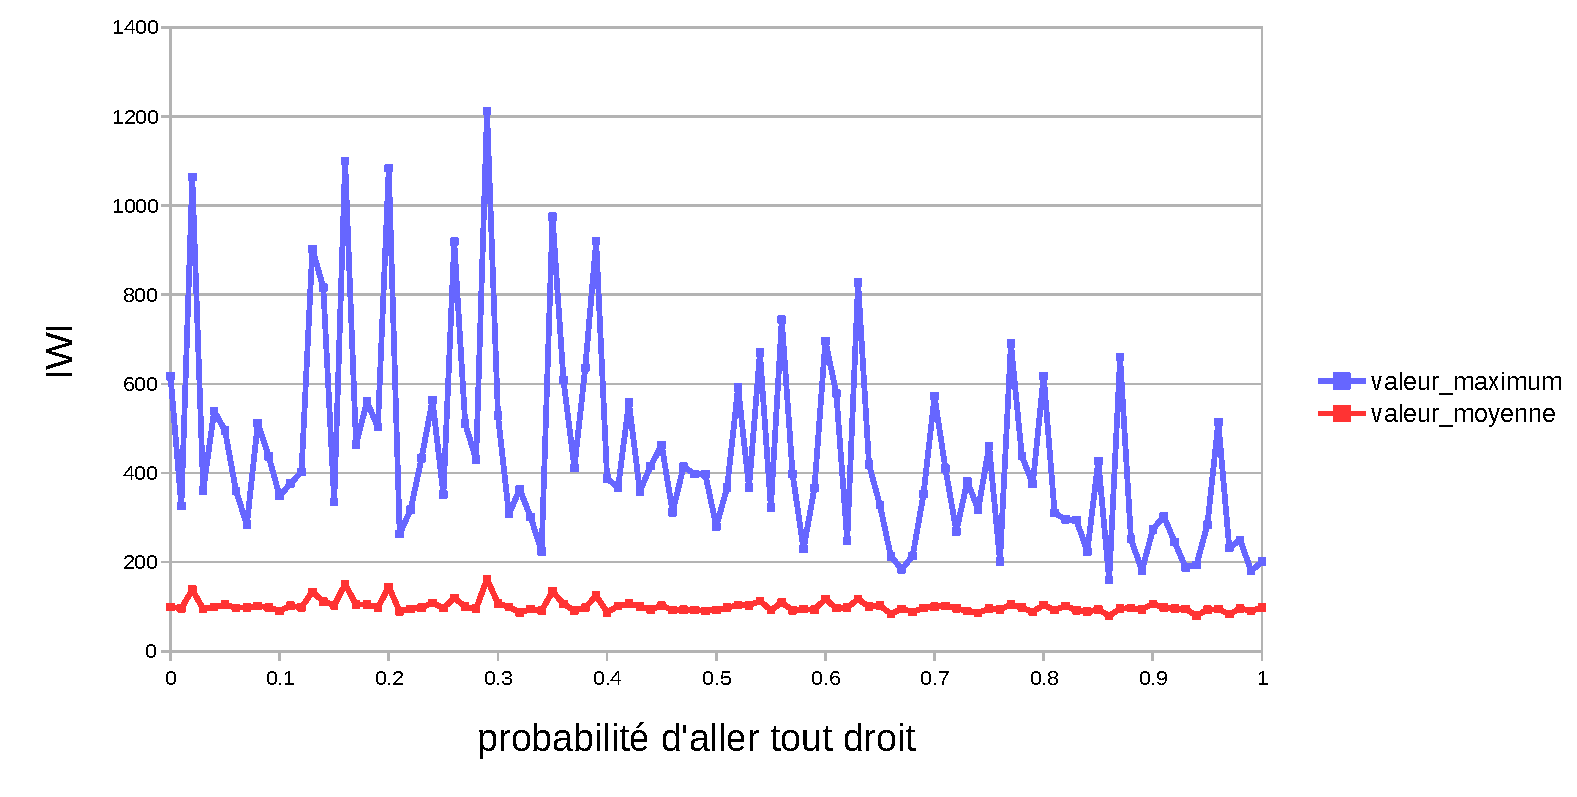
\includegraphics[width = 0.82\textwidth]{graphes pdf/variance go-ahead IWI spirale.pdf}
            \caption{IWI en fonction de $p_{avant}$ pour l'environnement en spirale}
        \end{center}
    \end{figure}
    \newpage
    \subsubsection{Environnement en corridor}
    \paragraph{}On observe que les tendances moyennes d'IGI et d'IWI reste stable avec la variation de $p_{avant}$. La forme spéciale de cet environnement tend à faire baisser les valeurs maximales d'IGI et d'IWI lorsque $p_{avant}$ tend  vers 1.
    Si la probabilité d'aller tout droit augmente, de nouvelles zones qui n'ont pas été visitée vont être atteintes plus vite par les agents, ce qui contribue à baisser IGI et IWI.
    \begin{figure}[!h]
        \begin{center}
            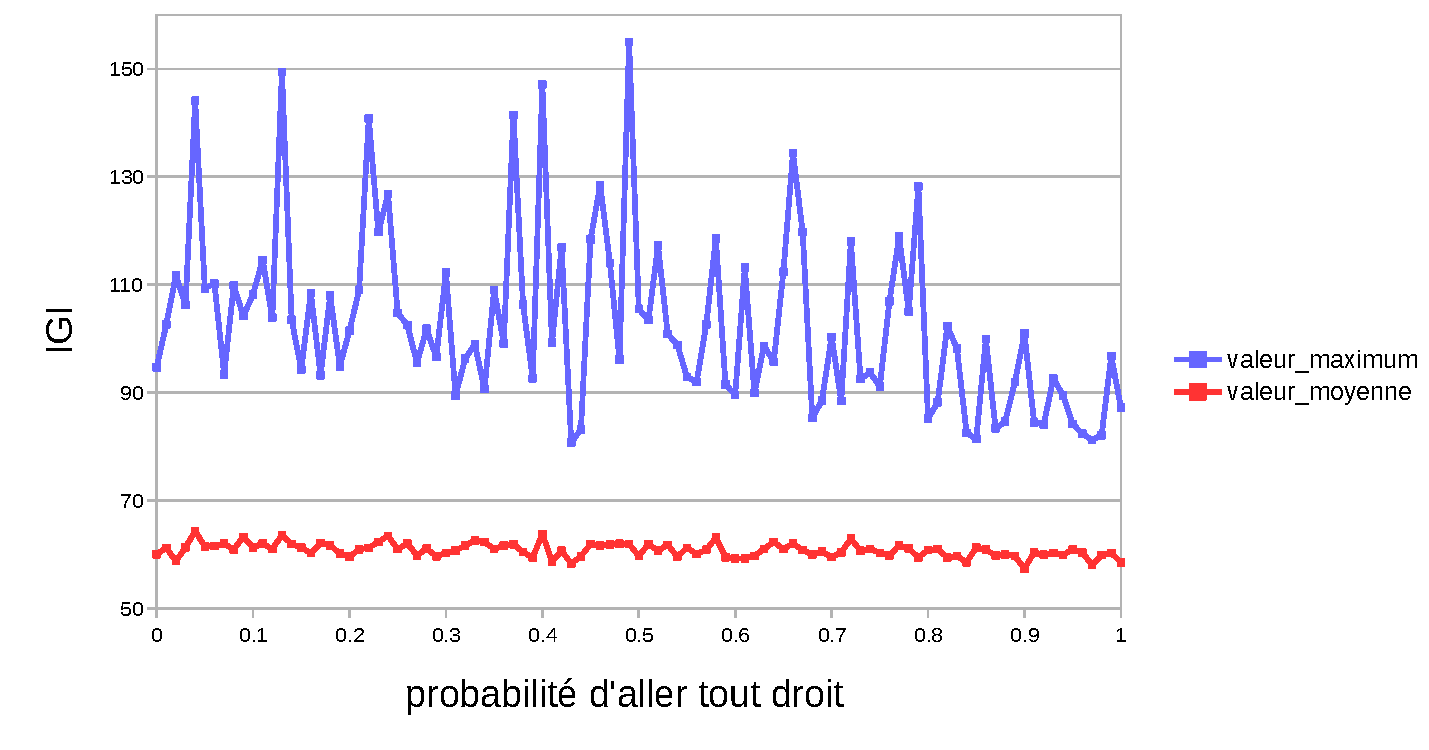
\includegraphics[width = 0.82\textwidth]{graphes pdf/variance go-ahead IGI corridor.pdf}
            \caption{IGI en fonction de $p_{avant}$ pour l'environnement en corridor}
        \end{center}
    \end{figure}
    \begin{figure}[!h]
        \begin{center}
            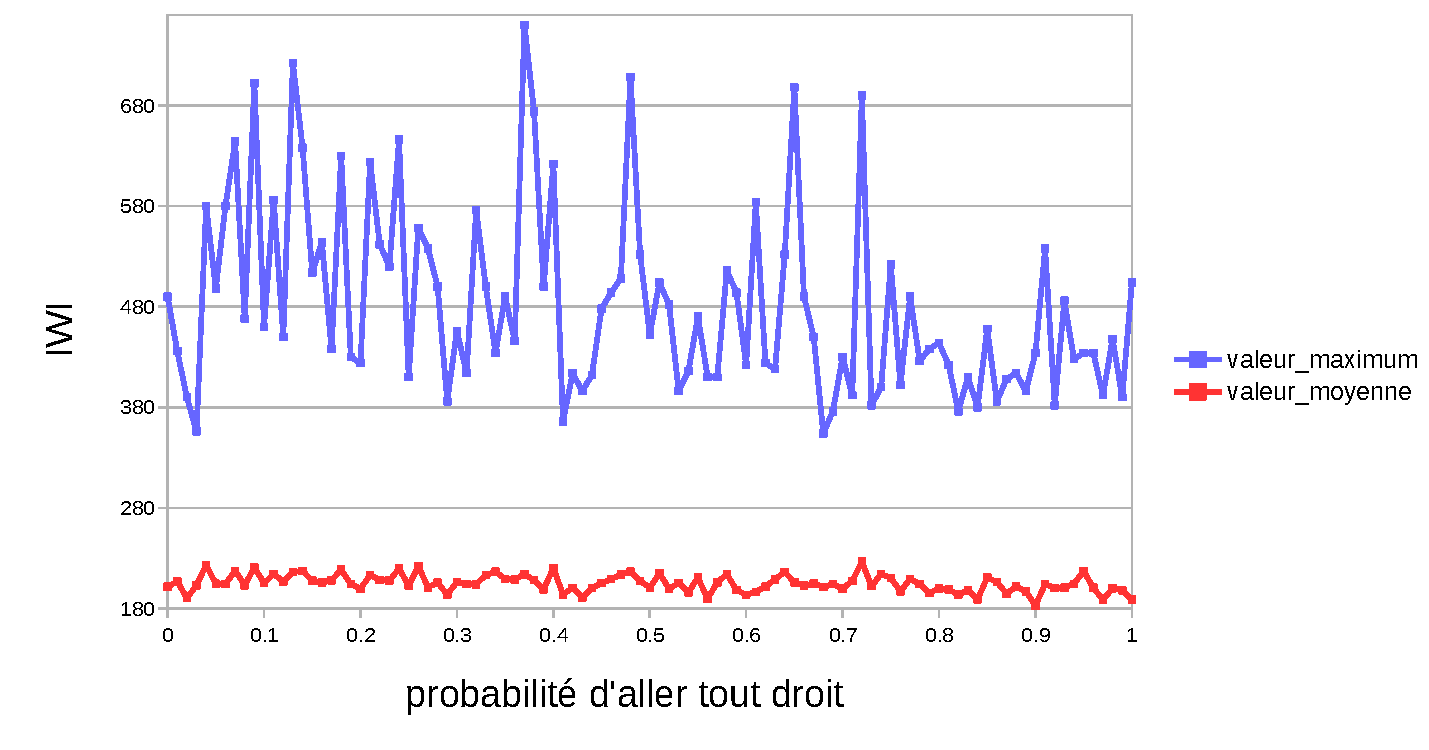
\includegraphics[width = 0.82\textwidth]{graphes pdf/variance go-ahead IWI corridor.pdf}
            \caption{IWI en fonction de $p_{avant}$ pour l'environnement en corridor}
        \end{center}
    \end{figure}
    \newpage
\section{Conclusion}
\paragraph{} Dans cet article, nous avons traité du problème de la patrouille dans un environnements inconnu.
Nous avons étudié l'impact des deux paramètres de notre modèle sur l'efficacité de la patrouille. Nous avons pu remarquer que 
l'intérêt de l'ajout d'agents supplémentaires varie en fonction de l'environnement. De même, la valeur de $p_{avant}$ a une influence sur la 
qualité de la patrouille dépendant de la configuration du terrain.

Il est possible de compléxifier ce modèle. On pourrait ainsi introduire la possibilité de paramétrer le champ de vision des agents, afin de pouvoir l'étendre à plus que les cases directement voisines de celles où ces derniers se trouvent.
Le phénomène d'évaporation des phéromones pourrait aussi être couplé à un phénomène de diffusion sur les cases environnantes, de sorte qu'à chaque pas de temps, une partie des phéromones évaporés aille s'ajouter à la quantité de phéromones des cases voisines.
Piste d'amélioration
    -> augmentation de la vision des agents
    -> diffusion des phéromones aux cases voisines
    -> ?
\appendix
\section{Annexe}
\listoffigures
\section*{Bibliographie}
\begin{thebibliography}{1}
    \bibitem{Swarm Approaches for the Patrolling Problem, Information Propagation vs. Pheromone Evaporation}
    Hoang-Nam Chu, Arnaud Glad, Olivier Simonin, François Sempé, Alexis Drogoul, François Charpillet.
    \textit{Swarm Approaches for the Patrolling Problem, Information Propagation vs. Pheromone Evaporation}
    Tools with Artificial Intelligence, 2007.
\end{thebibliography}

\end{document}